% DRAFT section for the FEM chapter — bone remodeling & the mechano-biological vicious cycle.
% Working draft for Overleaf paste/adaptation; NOT the canonical thesis source. Numbers are the
% actual verified outputs (2026-06-20). Citations use keys from refs.bib / docs/references.bib.
% Related-work prose: notes/fem_bone_remodeling_related_work_2026-06-20.md.

\section{Bone remodeling and the mechano-biological vicious cycle}
\label{sec:bone_remodeling}

\subsection{Bone constitutive model and density--modulus relations}
The peri-implant bone is modelled as a two-layer continuum (cortical shell, $E=13.7$~GPa; cancellous
core, $E=1.0$~GPa; $\nu=0.3$), consistent with the standard dental-implant FEM literature
\citep{GengTanLiu2001,Himmlova2004}. Where an apparent-density field is required, the standard
power-law relations $E=a\,\rho^{b}$ are used: Carter--Hayes ($E\propto\rho^{3}$) \citep{CarterHayes1977},
the site-specific Morgan law \citep{Morgan2003}, and the Keyak piecewise CT relation \citep{Keyak1998};
see \citet{Helgason2008} for the review. A patient-specific Hounsfield$\rightarrow$density calibration
is not performed (no scanner-calibrated CT was available), so region-wise literature moduli are used,
the standard fallback.

\subsection{Three equivalent remodeling formulations}
We employ the bone-adaptation law in three standard forms that we show to be mutually consistent.

\paragraph{Huiskes site-specific (SED).} The stimulus is the strain-energy density per unit mass
$S=U/\rho$, driven toward a site reference with a symmetric lazy zone \citep{Huiskes1987,Weinans1992}.

\paragraph{Frost mechanostat (microstrain).} The effective strain field is classified into Frost's
windows---disuse ($<\!100~\mu\varepsilon$), adapted ($100$--$1500~\mu\varepsilon$), formation
($1500$--$3000~\mu\varepsilon$), and \emph{pathological overload} ($>\!3000~\mu\varepsilon$)
\citep{Frost1987,Frost2003}. Crucially, the \emph{dual-threshold} form adds an upper bound: above
$\mathrm{MES_p}\!\approx\!3000~\mu\varepsilon$ bone is resorbed rather than apposed. This is what makes
the stress-concentrated implant crest \emph{lose} bone rather than densify---reproducing the clinical
crestal localisation of marginal bone loss \citep{Oh2002} from mechanics alone.

\paragraph{Mechanistic RANKL/OPG.} A reduced Lemaire/Pivonka osteoclast--osteoblast--bone ODE whose
master switch is the RANKL:OPG ratio, with inflammation (dysbiosis-driven) and mechanical overload as
the two RANKL drivers and TGF-$\beta$ coupling for homeostasis.

\paragraph{Equivalence.} Writing the RANKL/OPG law as a one-sided graded-threshold mechanostat, its
steady-state density field coincides with the Huiskes update to $|\Delta\rho|/|\rho|\approx0.04\%$
across physiological load, stress shielding, and hyper-load; the hard-threshold limit recovers the
Huiskes/Frost law exactly. The phenomenological law is therefore a limiting case of the mechanistic
model, letting the analysis speak both the examiner-standard (Huiskes/Frost) and the
mechanistic-contribution (RANKL/OPG) language from one model.

\subsection{FEM-coupled remodeling on the 3-D crown field}
Applying the Frost microstrain classification to the converged $\sim$245{,}000-element crowned-implant
field, the pathological-overload window ($>\!3000~\mu\varepsilon$) is confined almost entirely to the
peri-implant crest: $9.4\%$ of crestal ($0$--$3$~mm) bone vs.\ $\approx\!0\%$ deeper. The crestal
cortical von-Mises stress (p95 $\approx 22.6$--$29~\mathrm{MPa}$ under $100$~N at $30^\circ$) lies within
the reported $10$--$50$~MPa band \citep{GengTanLiu2001,Baggi2008,Gosai2024} at a safety factor
$\approx\!4\times$ below cortical yield---physiologically plausible and slightly conservative.
(Far-field alveolar bone shows apparent disuse, an artifact of loading only the implant; the
remodeling interpretation is restricted to the $r\le4$~mm peri-implant collar.)

\subsection{The mechano-biological vicious cycle}
\begin{figure}[t]
  \centering
  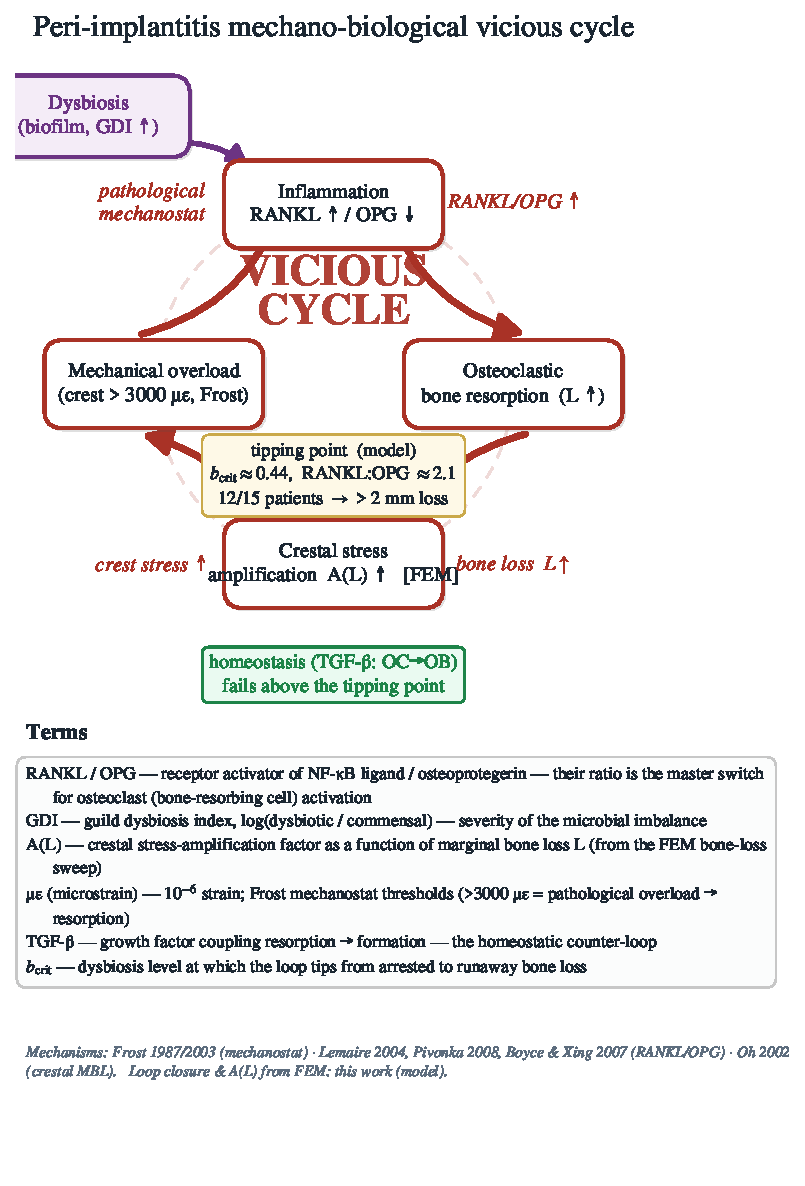
\includegraphics[width=0.74\linewidth]{figures/fig_vicious_cycle_en}
  \caption{The peri-implantitis mechano-biological vicious cycle. Dysbiosis drives inflammation,
  which through the RANKL:OPG switch \citep{BoyceXing2007,Lemaire2004,Pivonka2008} activates
  osteoclastic bone resorption; the resulting marginal bone loss $L$ raises the crestal
  stress-amplification factor $A(L)$ (from the FEM bone-loss sweep), pushing the crest into Frost's
  pathological-overload window ($>3000~\mu\varepsilon$) \citep{Frost1987,Frost2003}, which feeds back
  into RANKL. Bone loss initiates crestally, consistent with the clinical consensus \citep{Oh2002}.
  A homeostatic TGF-$\beta$ counter-loop balances the system below, and fails above, the tipping
  point. The loop closure, the FEM amplification $A(L)$, and the tipping-point values are model
  results of this work (calibration-dependent), not measured quantities.}
  \label{fig:vicious_cycle}
\end{figure}
The mechanical and biological channels close into a feedback loop (Fig.~\ref{fig:vicious_cycle}):
marginal bone loss $L$ raises the
crestal stress-amplification factor $A(L)$ (taken from the FEM bone-loss sweep), which adds to RANKL;
elevated RANKL:OPG drives osteoclastic resorption and further loss. The coupled model exhibits an
\emph{emergent tipping point}: above a dysbiosis threshold ($b_{\mathrm{crit}}\approx0.44$, RANKL/OPG
$\approx2.1$) the loss trajectory switches from arrested to progressive, with $12/15$ simulated patients
exceeding the $2$~mm peri-implantitis threshold over $36$~months. This bistability---rather than the
FEM stress map alone---is the work's distinctive contribution: the FEM$\leftrightarrow$clinical stress
co-localisation is well established \citep{Oh2002,Chang2018} and serves as grounding, whereas the
dysbiosis$\rightarrow$inflammation$\rightarrow$loss$\rightarrow$stress feedback is novel.

\paragraph{Uncertainty quantification.} To move the tipping behaviour beyond a single deterministic
trajectory, the cascade parameters are assigned literature-anchored priors (cytokine resolution,
osteoclast turnover, RANKL/OPG Hill exponent, mechanical synergy $\lambda$, and a resorption rate
calibrated to $\sim$0.3~mm/yr early progression) and propagated by Monte-Carlo ($N=600$) together with
the per-patient GDI scatter. This yields, per patient, a median 36-month bone-loss prediction with a
90\% credible band and a probability of crossing the mechanical point-of-no-return
(Fig.~\ref{fig:uq}); the cohort separates into low- and high-risk groups rather than a single curve.
A global sensitivity analysis (Spearman $\rho$ of each parameter against 36-month loss) ranks the
osteoclast formation/turnover rates ($k_C,g_C$; $|\rho|\approx0.5$) and the resorption gain ($k_L$)
above the mechanical synergy ($\lambda$; $|\rho|\approx0.26$): the loop is biology-dominated with a
moderate, non-negligible mechanical contribution, and the ranking identifies which quantity to
measure next to tighten the prediction. The tipping point thus persists across the physiological
prior range (robust), while its exact location remains calibration-dependent (honest scope).

\begin{figure}[t]
  \centering
  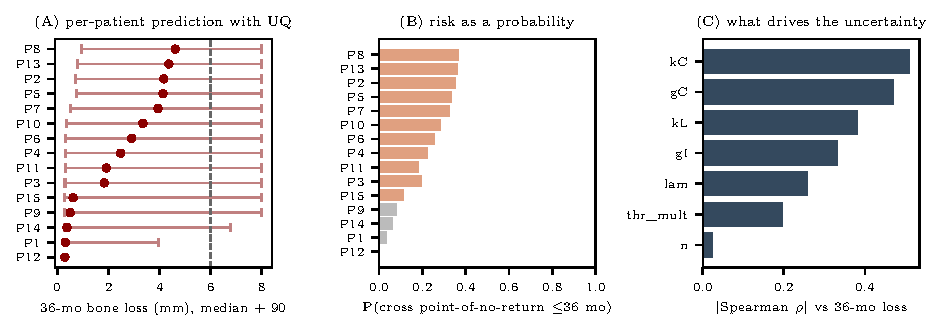
\includegraphics[width=\linewidth]{figures/fem_periimplantitis_uq}
  \caption{Uncertainty quantification of the peri-implantitis cascade. (A) Per-patient 36-month
  bone-loss prediction: median (dot) with 90\% credible band, driven by the measured GDI(t) of each
  patient under Monte-Carlo sampling of literature-anchored priors; the dashed line is the mechanical
  point-of-no-return. (B) The same risk expressed as the probability of crossing that point within
  36~months. (C) Global sensitivity (|Spearman $\rho$| of each parameter against 36-month loss): the
  osteoclast formation/turnover rates ($k_C,g_C$) and resorption gain ($k_L$) dominate, above the
  mechanical synergy ($\lambda$) and Hill exponent ($n$).}
  \label{fig:uq}
\end{figure}

\subsection{Clinical grounding (qualitative)}
Validation follows the field norm of spatial co-localisation rather than quantitative longitudinal
density fitting (only $\sim$9\% of implant-FEA studies validate at all \citep{Chang2018}). The predicted
crestal concentration of remodeling activity matches the clinical consensus that bone loss begins
crestally \citep{Oh2002}; the simulated progressive-loss magnitude ($>\!2$~mm) and the healthy
steady-state ($<\!0.2$~mm/yr \citep{Albrektsson1986}) bracket the clinical range. A quantitative
per-patient density validation would require the longitudinal radiographic data discussed in the
Outlook.
